\chapter{User Interface Design}
\label{cha:ui}
In this section, we will show an overall view of the different user interfaces of Travlendar+.
It shows either user flow and the different screens of the application. (Figure \ref{fig:generaluxdiag})
\newline
Being compliant with the requirements in the RASD document, in figure \ref{fig:mobileuxdiag} we are showing as well a mobile implementation integrating the user flow across Travlendar+.
\newline
The general UX Diagram is composed of 2 parts:
\begin{itemize}
	\item the \textbf{white} one describes the common functionalities of the web and mobile implementation
	\item the \textbf{yellow} one describes the functionalities implemented only by the mobile client,
\end{itemize}


\begin{figure}
	\centering
	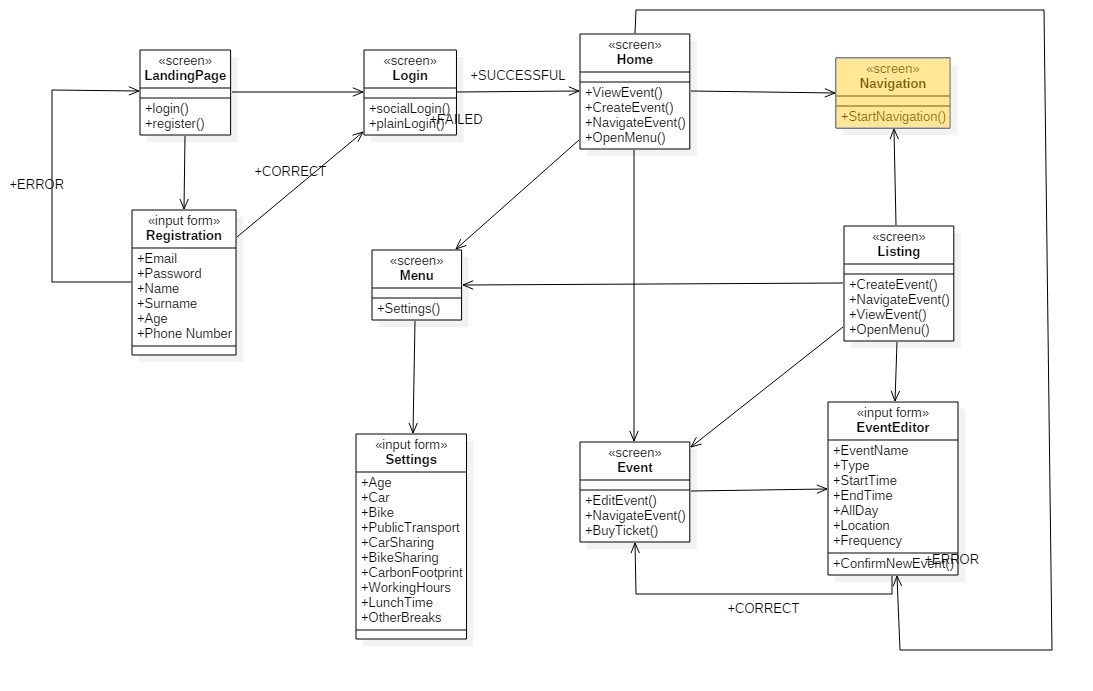
\includegraphics[width=6in]{./diagrams/GeneralUxDiagram.jpg}
	\caption{UX Diagram of the client implementation.}
	\label{fig:generaluxdiag}
\end{figure}
\begin{figure}
	\centering
	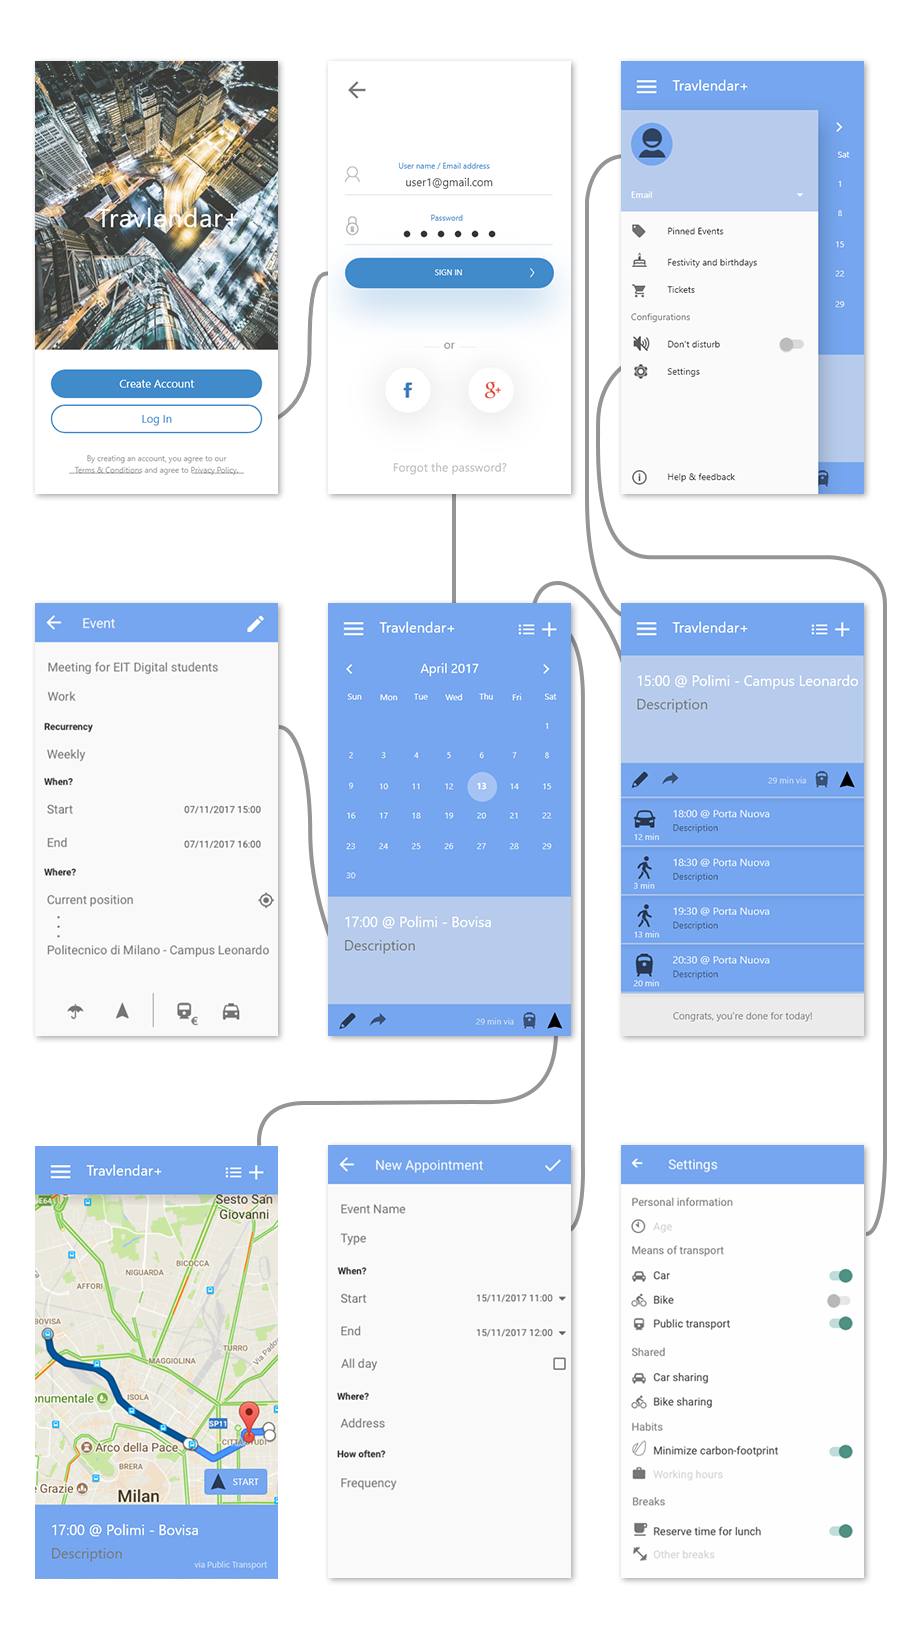
\includegraphics[width=5in]{./diagrams/MobileUxDiagram.png}
	\caption{UX Diagram for the mobile implementation.}
	\label{fig:mobileuxdiag}
\end{figure}